\documentclass[12pt]{article}

\usepackage{report}

\usepackage[utf8]{inputenc} % allow utf-8 input
\usepackage[T1]{fontenc}    % use 8-bit T1 fonts
\usepackage[colorlinks=true, linkcolor=black, citecolor=blue, urlcolor=blue]{hyperref}       % hyperlinks
\usepackage{url}            % simple URL typesetting
\usepackage{booktabs}       % professional-quality tables
\usepackage{amsfonts}       % blackboard math symbols
\usepackage{nicefrac}       % compact symbols for 1/2, etc.
\usepackage{microtype}      % microtypography
\usepackage{lipsum}		% Can be removed after putting your text content
\usepackage{graphicx}
\usepackage{natbib}
\usepackage{doi}
\usepackage{listings}
\usepackage{xcolor}
\usepackage{float}
\setcitestyle{aysep={,}}



\title{Project Step 2}

\author{Brian Lee, Chloe Gentry, Vinny Rose\\
\AND\\
\AND
\AND
\AND
\AND
	CS.3339 Computer Architecture\\
\AND
	Texas State University\\
}

% Uncomment to remove the date
\date{October 28, 2024}

% Uncomment to override  the `A preprint' in the header
\renewcommand{\headeright}{Project Step 2 - Group Name}
\renewcommand{\undertitle}{Smarty Pants}
\renewcommand{\shorttitle}{}

\definecolor{codegreen}{rgb}{0,0.6,0}
\definecolor{codegray}{rgb}{0.5,0.5,0.5}
\definecolor{codepurple}{rgb}{0.58,0,0.82}
\definecolor{backcolour}{rgb}{0.95,0.95,0.92}

\lstdefinestyle{mystyle}{
    backgroundcolor=\color{backcolour},   
    commentstyle=\color{codegreen},
    keywordstyle=\color{magenta},
    numberstyle=\tiny\color{codegray},
    stringstyle=\color{codepurple},
    basicstyle=\ttfamily\footnotesize,
    breakatwhitespace=false,         
    breaklines=true,                 
    captionpos=b,                    
    keepspaces=true,                 
    numbers=left,                    
    numbersep=5pt,                  
    showspaces=false,                
    showstringspaces=false,
    showtabs=false,                  
    tabsize=2
}

\lstset{style=mystyle}


\begin{document}
\maketitle

\newpage
\tableofcontents
\thispagestyle{empty}


\newpage
\setcounter{page}{1}
\section{Introduction}
For step 1 we were assigned to design 4 computer circuits. A 1-bit Nand circuit, 1-bit Nor circuit, 1-bit Not circuit, and a 1x4 shifting circuit. We used Verilog to define the code for the circuits and GTKWave to simulate the waveforms for the circuits.

\section{2x4 Shift Circuit}
\label{sec:headings}

The 1x4 shift circuit takes a 4-bit input and shifts the bits to the left or right based on a control signal. This shifting operation moves each bit in the input to an adjacent position, with the vacant positions being filled by zeros. 

\subsection{Shift Circuit Verilog Code}
\lstinputlisting[language=Verilog]{2x2x4Shifter/shift_tb.v}

To test the Shift circuit we have created 2 registers, one for the input and one for the shifting then one wire for the output. If this circuit works properly the output should display the input shifted to the left and zeros filling the shifted positions.
\lstinputlisting[language=Verilog]{1x4bit-shift/shift_tb.v}


\subsection{Shift Circuit Waveforms}

At 0 ns, we can see that A is 0, so the output Y is 0.
\begin{figure}[H]
    \centering
    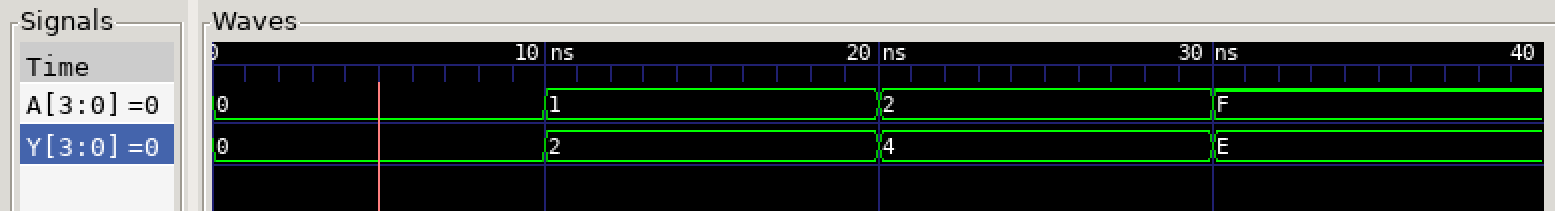
\includegraphics[width = 1.0\textwidth]{1x4bit-shift/shift_wave1.PNG}
    \caption{Shift Circuit with marker at 0ns}
    \label{fig:shift-wave1}
\end{figure}

At 10 ns, A is 1 (0001), so Y becomes 2 (0010).
\begin{figure}[H]
    \centering
    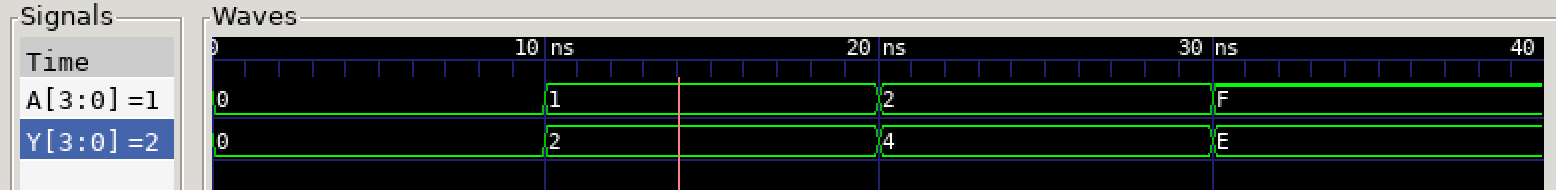
\includegraphics[width = 1.0\textwidth]{1x4bit-shift/shift_wave2.PNG}
    \caption{Shift Circuit with marker at 10ns}
    \label{fig:shift-wave2}
\end{figure}

At 20 ns, A is 2 (0010), so Y becomes 4 (0100).
\begin{figure}[H]
    \centering
    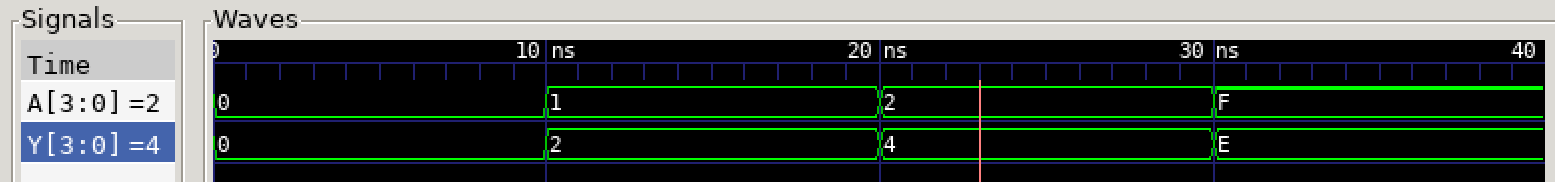
\includegraphics[width = 1.0\textwidth]{1x4bit-shift/shift_wave3.PNG}
    \caption{Shift Circuit with marker at 20ns}
    \label{fig:shift-wave3}
\end{figure}


At 30 ns, A is F (1111) so Y becomes E (1110).
\begin{figure}[H]
    \centering
    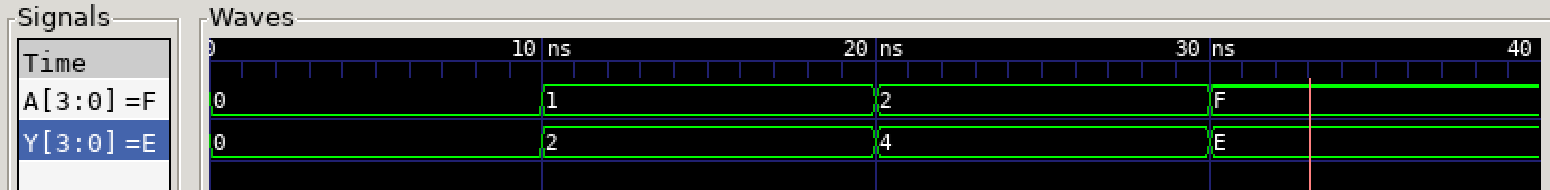
\includegraphics[width = 1.0\textwidth]{1x4bit-shift/shift_wave4.PNG}
    \caption{Shift Circuit with marker at 30ns}
    \label{fig:shift-wave4}
\end{figure}

\section{Not Circuit}
The Not circuit takes one input A, with an output Y. This will output a 0 if A is a 1, and will output 1 if A is a 0.

```\begin{figure}[H]
    \centering
    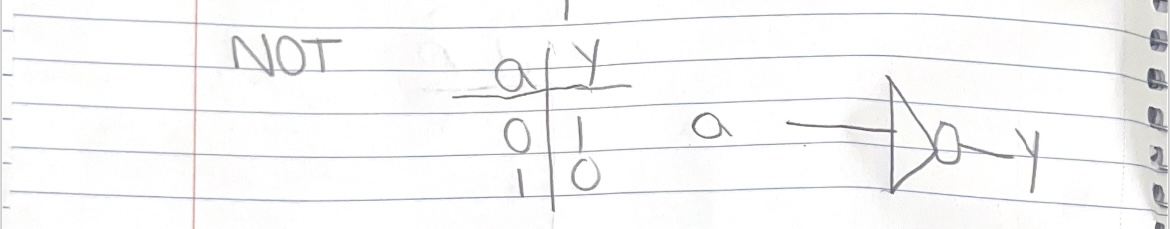
\includegraphics[width = 1.0\textwidth]{Truth-Tables/NotTT.PNG}
    \caption{Not truth table and gate}
    \label{fig:shift-table}
\end{figure}

\subsection{Not Circuit Verilog Code}
\lstinputlisting[language=Verilog]{not/not_gate.v}

To test the Not circuit, we have created one register A, as well as a wire Y. This way we are able to take each input for A and test output for A=0 and A=1. We'll know if this is working correctly if Y returns 1 for the test where A is 0 and Y returns 0 when A is 1.
\lstinputlisting[language=Verilog]{not/not_tb.v}

\subsection{Not Circuit Waveform}
At 2 ns, we can see that  A is 0, so the output Y is 1.
\begin{figure}[H]
    \centering
    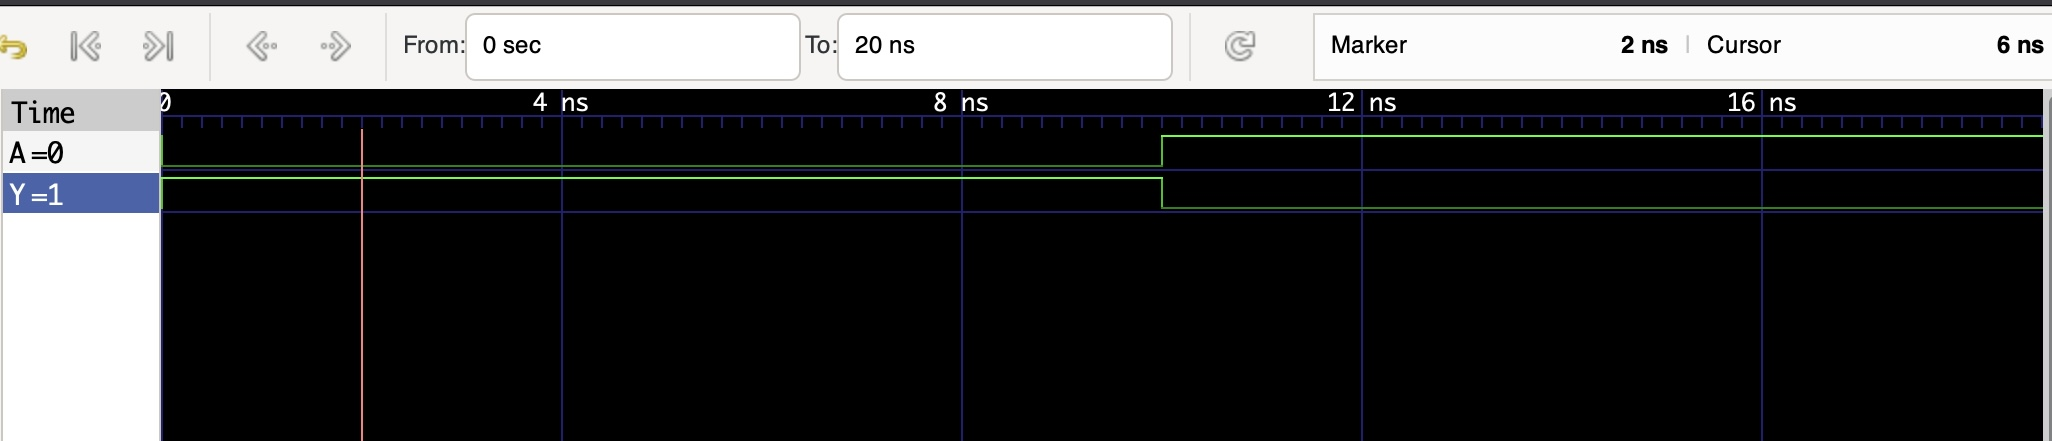
\includegraphics[width = 1.0\textwidth]{not/not_wave.PNG}
    \caption{Not Circuit with marker at 2ns}
    \label{fig:enter-label}
\end{figure}

At 10 ns, A becomes 1, so Y becomes 0.
\begin{figure}[H]
    \centering
    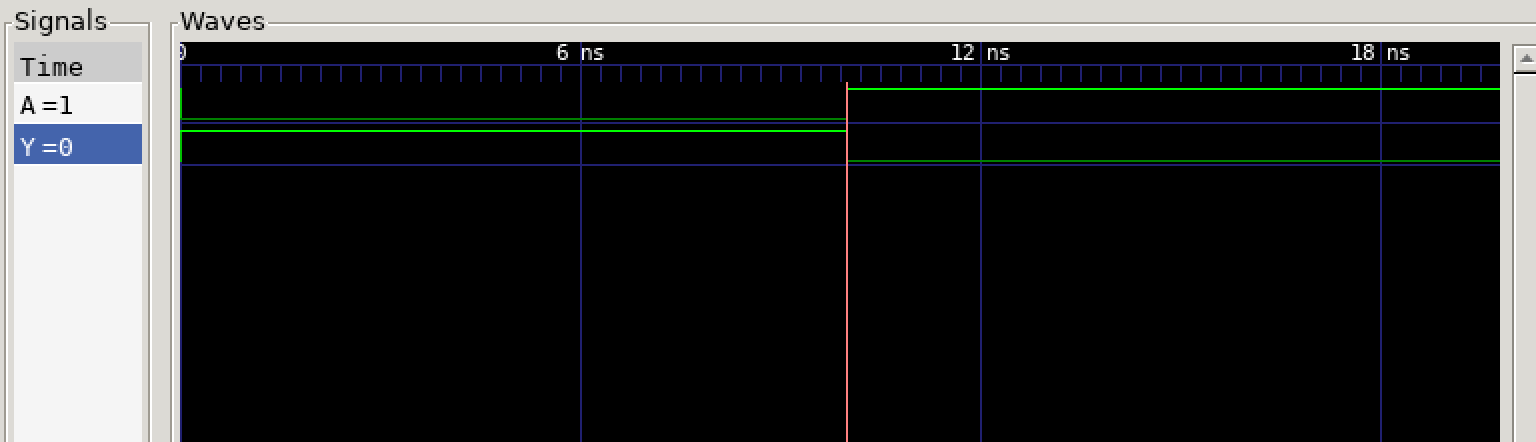
\includegraphics[width = 1.0\textwidth]{not/not_wave1.png}
    \caption{Not Circuit with marker at 10ns}
    \label{fig:enter-label}
\end{figure}

\section{Nand Circuit}
The Nand circuit takes two inputs, A and B, with an output Y. Nand will only give us back a 0 when A and B are both 1.

```\begin{figure}[H]
    \centering
    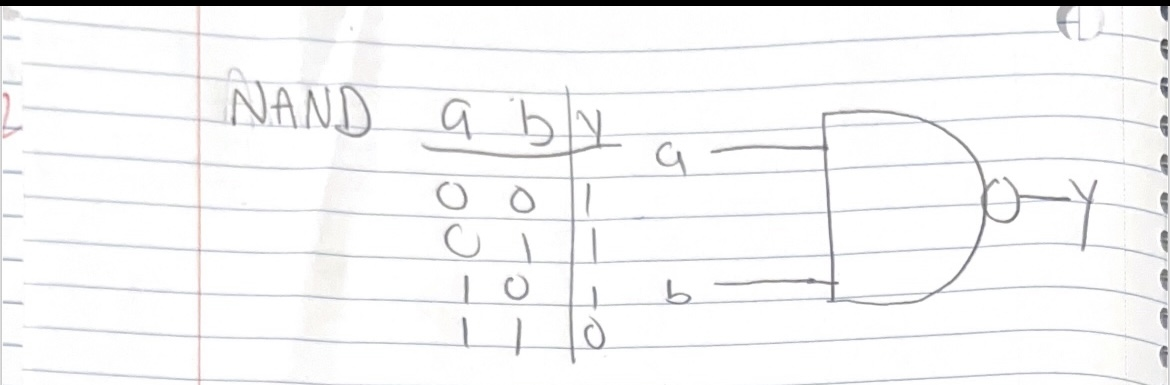
\includegraphics[width = 1.0\textwidth]{Truth-Tables/NandTT.PNG}
    \caption{Nand truth table and gate}
    \label{fig:shift-table}
\end{figure}

\subsection{Nand Circuit Verilog Code}
At 2 ns, we can see that  A is 0, so the output Y is 1.
\lstinputlisting[language=Verilog]{nand/nand_gate.v}

To test the Nand circuit, we have created two registers, A and B, as well as a wire Y. This allows us to test both inputs and one output. We'll know its correct if Y is 1 for all cases except where A and B are both 1.
\lstinputlisting[language=Verilog]{nand/nand_tb.v}
\subsection{Nand Circuit Waveform}

At 0 ns, A and B are 0, so Y is 1.
\begin{figure}[H]
    \centering
    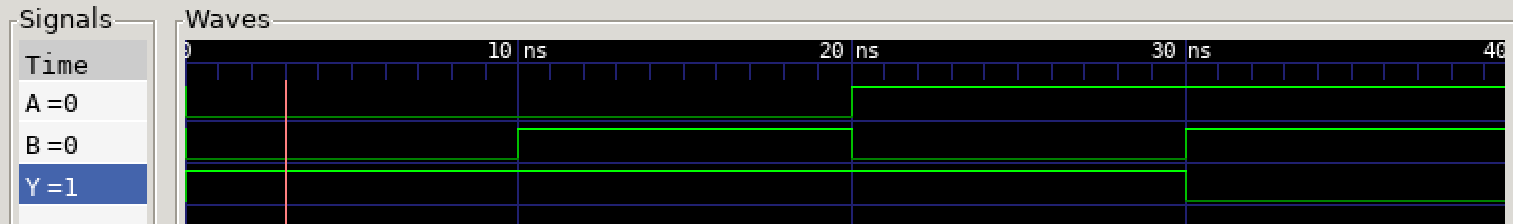
\includegraphics[width = 1.0\textwidth]{nand/nand_wave1.PNG}
    \caption{Nand Circuit with marker at 0ns}
    \label{fig:enter-label}
\end{figure}

At 10 ns, A is 0 and B is 1, so Y stays 1.
\begin{figure}[H]
    \centering
    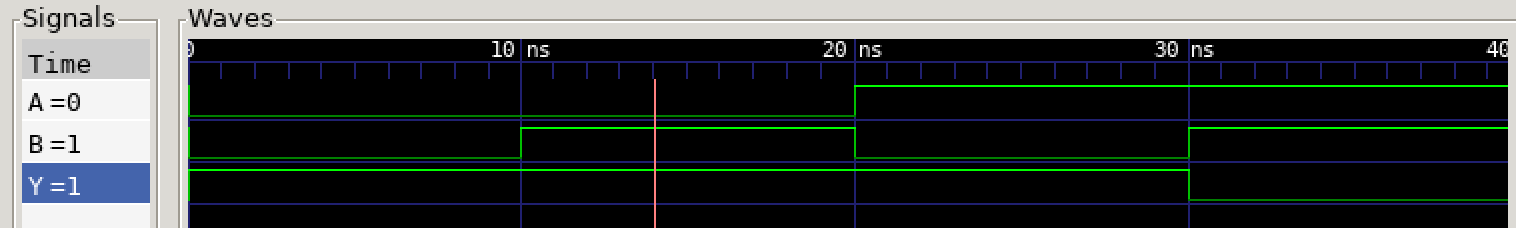
\includegraphics[width = 1.0\textwidth]{nand/nand_wave2.PNG}
    \caption{Nand Circuit with marker at 10ns}
    \label{fig:enter-label}
\end{figure}

At 20 ns, A is 1 and B is 0, so Y is still 1.
\begin{figure}[H]
    \centering
    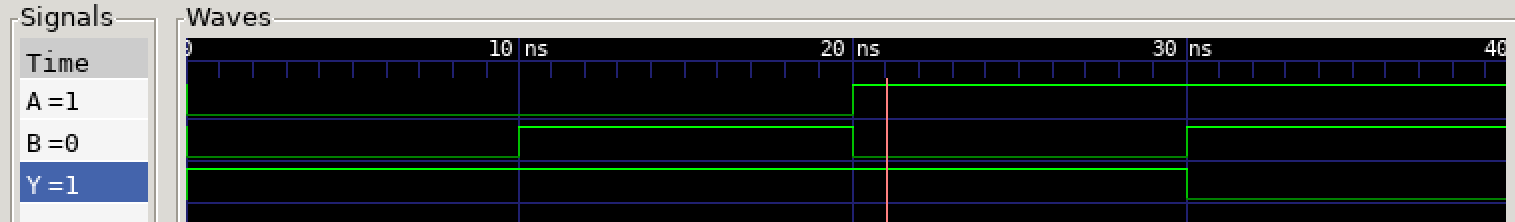
\includegraphics[width = 1.0\textwidth]{nand/nand_wave3.PNG}
    \caption{Nand Circuit with marker at 20ns}
    \label{fig:enter-label}
\end{figure}

At 30 ns, both A and B are 1, so Y finally flips to 0.
\begin{figure}[H]
    \centering
    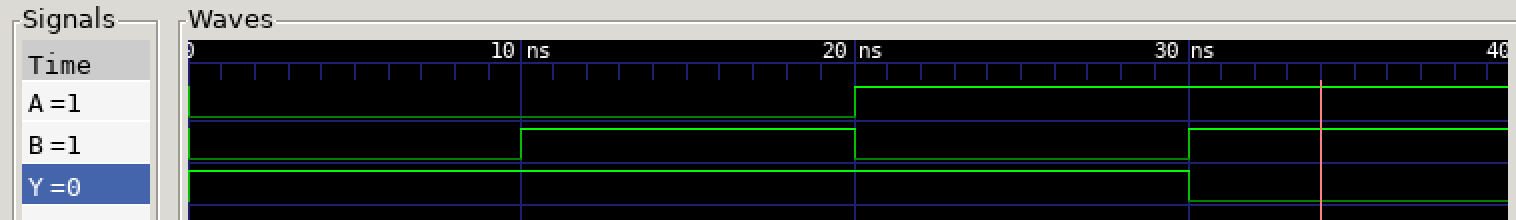
\includegraphics[width = 1.0\textwidth]{nand/nand_wave4.PNG}
    \caption{Nand Circuit with marker at 30ns}
    \label{fig:enter-label}
\end{figure}

\section{Nor Circuit}
The Nor circuit takes two inputs, A and B, with an output Y. This will output a 0 if either A or B is a 1, and will only output 1 if A and B are both 0.

```\begin{figure}[H]
    \centering
    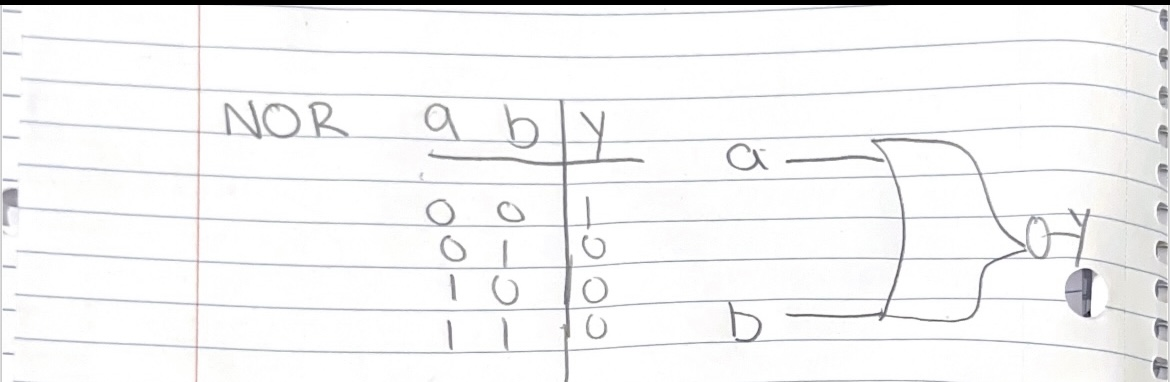
\includegraphics[width = 1.0\textwidth]{Truth-Tables/NorTT.PNG}
    \caption{Nor truth table and gate}
    \label{fig:shift-table}
\end{figure}

\subsection{Nor Circuit Verilog Code}
At 2 ns, we can see that  A is 0, so the output Y is 1.
\lstinputlisting[language=Verilog]{nor/nor_gate.v}

To test the Nor circuit, we have created two registers, A and B, as well as a wire Y. This way we are able to take two inputs at a time and test each possible input for the circuit. We'll know if this is working correctly if Y returns 1 for the test where A and B are 0 and Y should return 0 for the rest.
\lstinputlisting[language=Verilog]{nor/nor_tb.v}
\subsection{Nor Circuit Waveform}

At 0 ns, A and B are 0, so Y is 1.
\begin{figure}[H]
    \centering
    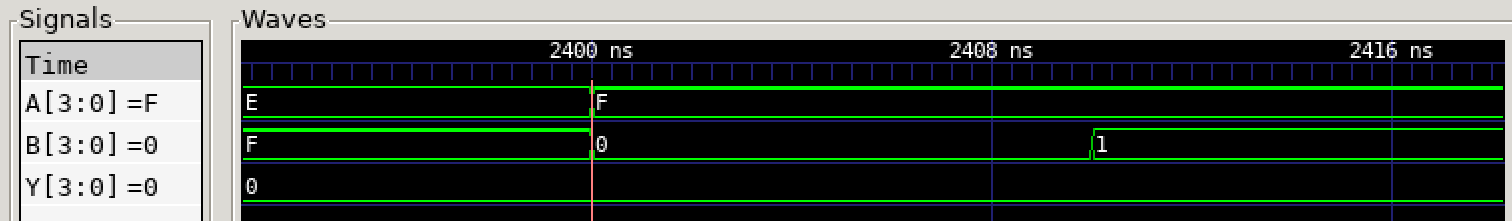
\includegraphics[width = 1.0\textwidth]{nor/nor_wave1.PNG}
    \caption{Nor Circuit with marker at 0ns}
    \label{fig:enter-label}
\end{figure}

At 10 ns, A is 0 and B is 1, so Y is now 0.
\begin{figure}[H]
    \centering
    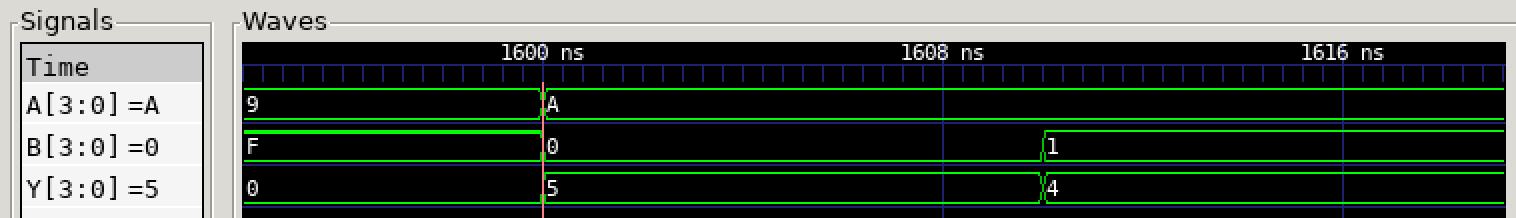
\includegraphics[width = 1.0\textwidth]{nor/nor_wave2.PNG}
    \caption{Nor Circuit with marker at 10ns}
    \label{fig:enter-label}
\end{figure}

At 20 ns, A is 1 and B is 0, so Y is still 0.
\begin{figure}[H]
    \centering
    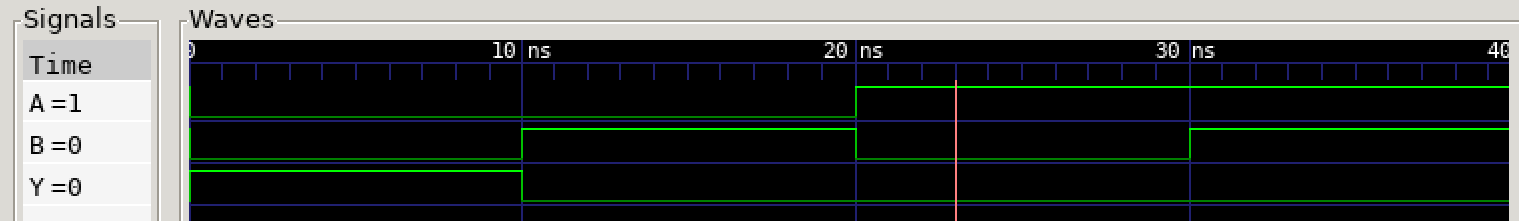
\includegraphics[width = 1.0\textwidth]{nor/nor_wave3.PNG}
    \caption{Nor Circuit with marker at 20ns}
    \label{fig:enter-label}
\end{figure}

At 30 ns, both A and B are 1, so Y again stays 0.
\begin{figure}[H]
    \centering
    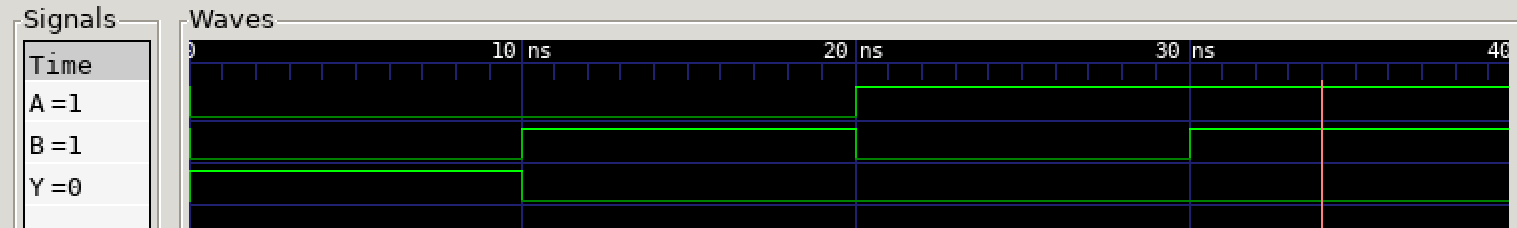
\includegraphics[width = 1.0\textwidth]{nor/nor_wave4.PNG}
    \caption{Nor Circuit with marker at 30ns}
    \label{fig:enter-label}
\end{figure}

\subsection{Nand Circuit}
The Nand circuit takes two 4-bit inputs A & B, with a 4-bit output Y. A & B will undergo the bitwise Nand operation, and the result will be output to Y.
\lstinputlisting[language=Verilog]{Nand/nand_gate.v} 

To test the Nand circuit, we have created two registers A & B, as well as a wire Y. We then create a for loop to produce all 16 possible values for A & B. We will know that our Nand circuit is behaving as expected if Y produces correct values for all combinations of A & B. For example, if A=0001 and B=0001, the expected result for Y is 1110. 
 \lstinputlisting[language=Verilog]{Nand/nand_tb.v}

\subsection{Nand Circuit Waveform} 

At 1ns, A & B are both 0000, so Y is F (1111).
\begin{figure}[h]
 \centering
 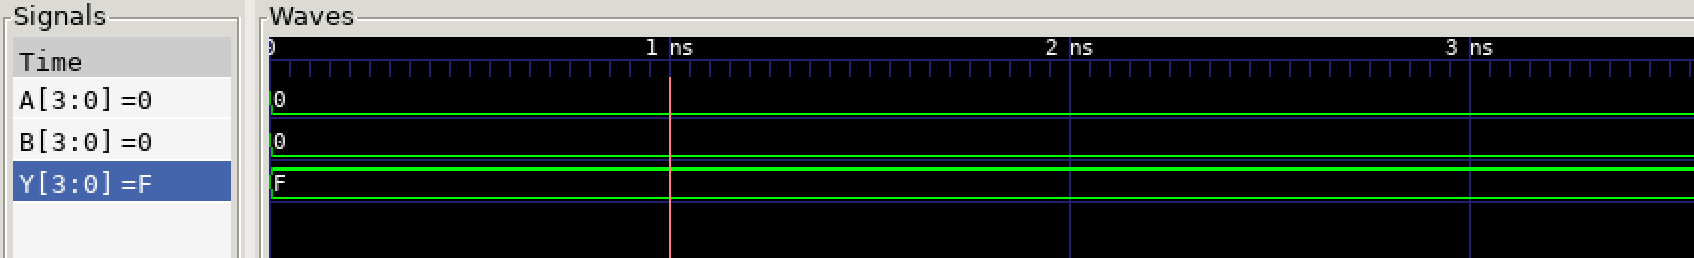
\includegraphics[width = 1.0\textwidth]{/Step2/Nand/nand_wave.png}
 \caption{Nand Circuit with marker at 1ns}
 \label{fig:enter-label} 
\end{figure} 

At 500ns, A=0011 and B=0010, so Y=D (1101) 
 \begin{figure}[h]
 \centering 
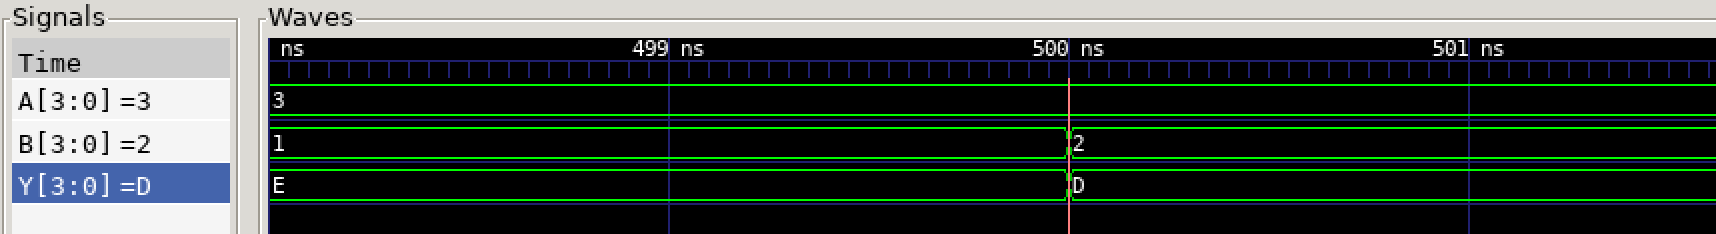
\includegraphics[width = 1.0\textwidth]{/Step2/Nand/nand_wave1.png}
 \caption{Nand Circuit with marker at 500ns}
 \label{fig:enter-label}
 \end{figure}

At 2500ns, A & B are both F (1111), so Y is 0000. 
 \begin{figure}[h]
 \centering 
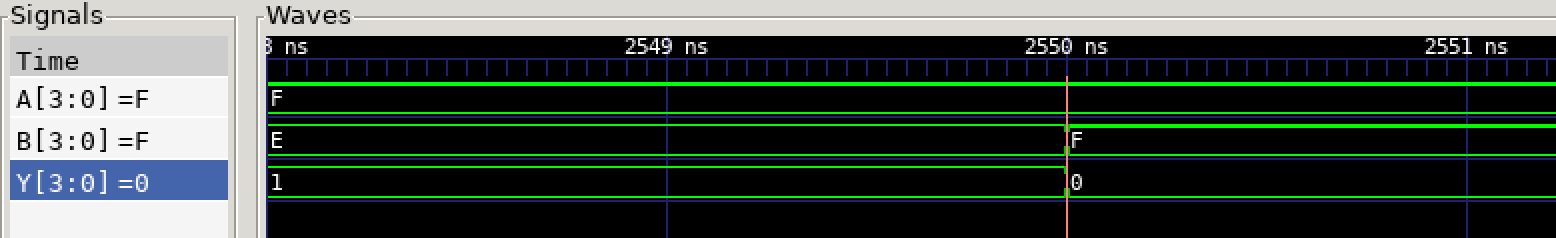
\includegraphics[width = 1.0\textwidth]{/Step2/Nand/nand_wave2.png}
 \caption{Nand Circuit with marker at 560ns}
 \label{fig:enter-label}
 \end{figure}


\subsection{And Circuit}
The And circuit takes two 4-bit inputs A & B, with a 4-bit output Y. A & B will undergo the bitwise And operation, and the result will be output to Y.
\lstinputlisting[language=Verilog]{And/and_gate.v} 

To test the And circuit, we have created two registers A & B, as well as a wire Y. We then create a for loop to produce all 16 possible values for A & B. We will know that our And circuit is behaving as expected if Y produces correct values for all combinations of A & B. For example, if A=0001 and B=0001, the expected result for Y is 0001. 
 \lstinputlisting[language=Verilog]{And/and_tb.v}

\subsection{And Circuit Waveform} 

At 1ns, A & B are both 0000, so Y is also 0000
\begin{figure}[h]
 \centering
 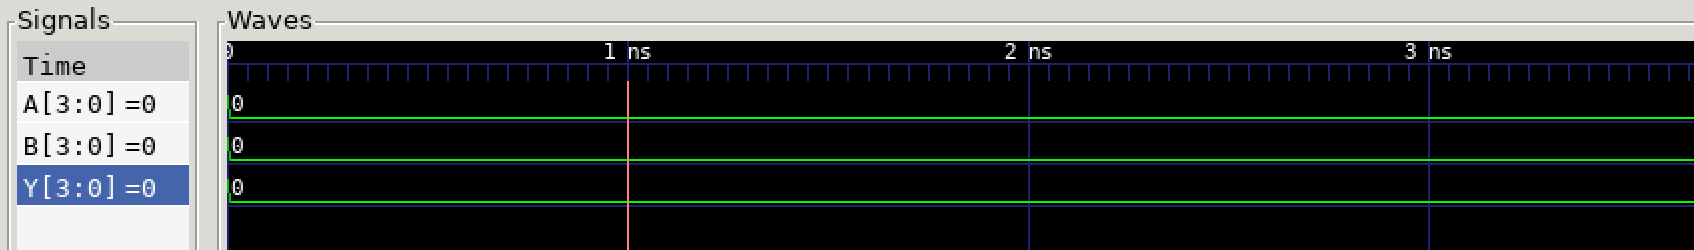
\includegraphics[width = 1.0\textwidth]{/Step2/And/and_wave.png}
 \caption{And Circuit with marker at 1ns}
 \label{fig:enter-label} 
\end{figure} 

At 500ns, A=0011 and B=0010, so Y=0010
 \begin{figure}[h]
 \centering 
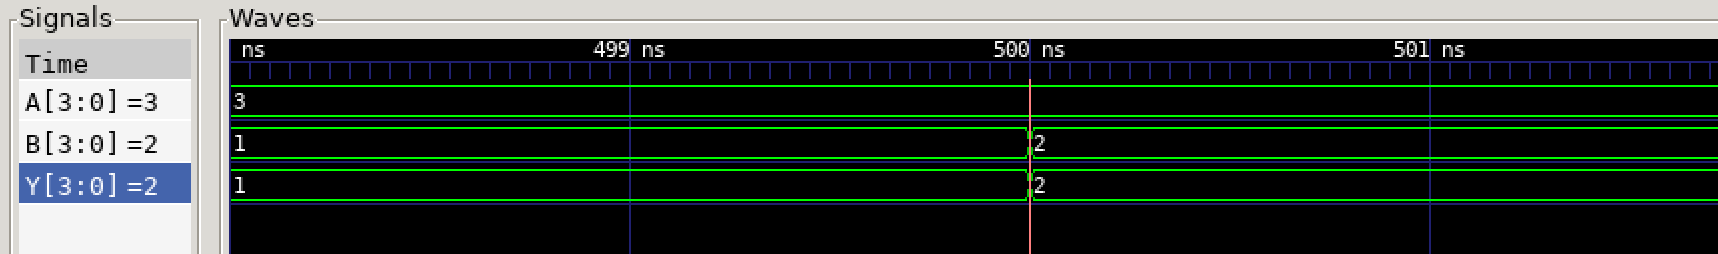
\includegraphics[width = 1.0\textwidth]{/Step2/And/and_wave1.png}
 \caption{And Circuit with marker at 500ns}
 \label{fig:enter-label}
 \end{figure}

At 2550ns, A & B are both F (1111), so Y is also F (1111).
 \begin{figure}[h]
 \centering 
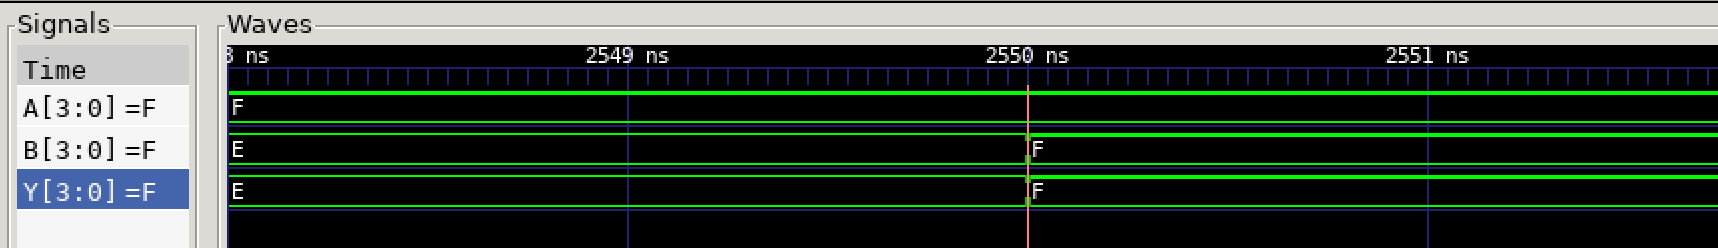
\includegraphics[width = 1.0\textwidth]{/Step2/And/and_wave2.png}
 \caption{And Circuit with marker at 2550ns}
 \label{fig:enter-label}
 \end{figure}

\subsection{Xor Circuit}
The Xor circuit takes two 4-bit inputs A & B, with a 4-bit output Y. A & B will undergo the bitwise Xor operation, and the result will be output to Y.
\lstinputlisting[language=Verilog]{Xor/xor_gate.v} 

To test the Xor circuit, we have created two registers A & B, as well as a wire Y. We then create a for loop to produce all 16 possible values for A & B. We will know that our Xor circuit is behaving as expected if Y produces correct values for all combinations of A & B. For example, if A=1010 and B=1101, the expected result for Y is 0111. 
 \lstinputlisting[language=Verilog]{Xor/xor_tb.v}

\subsection{Xor Circuit Waveform} 

At 1ns, A & B are both 0000, so Y is also 0000.
\begin{figure}[h]
 \centering
 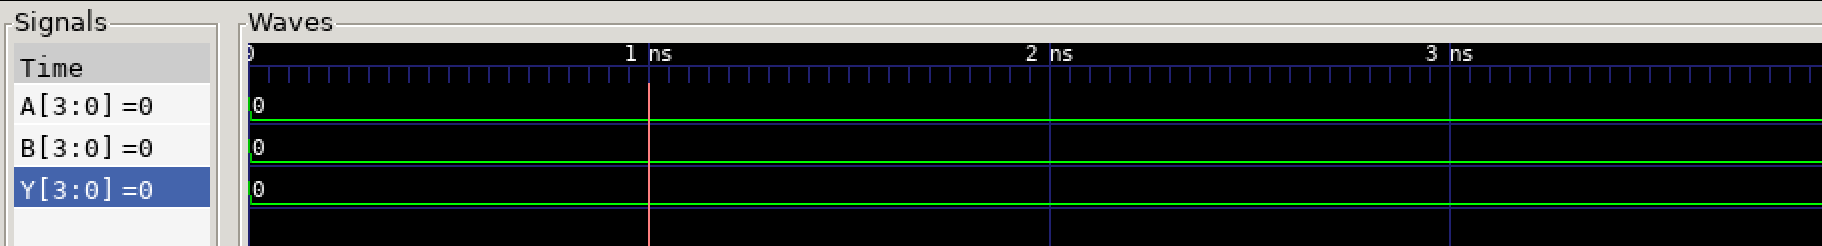
\includegraphics[width = 1.0\textwidth]{/Step2/Xor/xor_wave.png}
 \caption{Xor Circuit with marker at 1ns}
 \label{fig:enter-label} 
\end{figure} 

At 500ns, A=0011 and B=0010, so Y=0001.
 \begin{figure}[h]
 \centering 
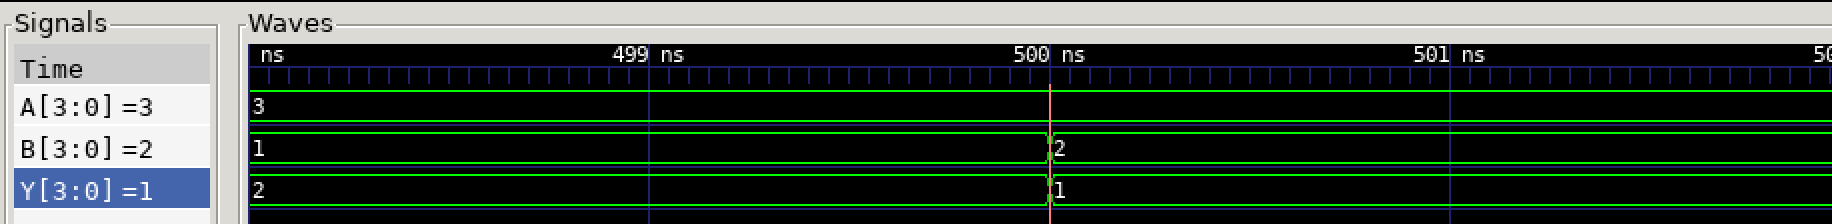
\includegraphics[width = 1.0\textwidth]{/Step2/Xor/xor_wave1.png}
 \caption{Xor Circuit with marker at 500ns}
 \label{fig:enter-label}
 \end{figure}

At 2500ns, A & B are both F, so Y=0000.
 \begin{figure}[h]
 \centering 
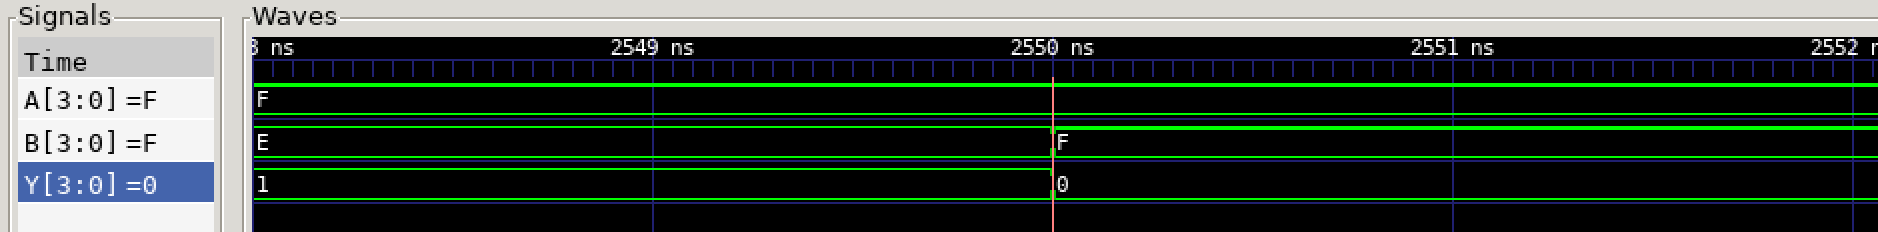
\includegraphics[width = 1.0\textwidth]{/Step2/Xor/xor_wave2.png}
 \caption{Xor Circuit with marker at 2500ns}
 \label{fig:enter-label}
 \end{figure}

\subsection{Addition Circuit}
The Addition circuit takes two 4-bit inputs A & B along with a 1-bit carry in to extend the output range from 15 to 31. The circuit’s outputs include  a 4-bit output called Sum, along with a 1-bit carry_out to accommodate the extended range. The has an intermediary 5-bit variable, full_sum, which is used to extract carry out and partial sum. First the full sum is found by adding A + B + carry_in. Then, Sum is assigned to the 4 lower bits of full_sum. Then, carry_out is assigned to the 5th bit of full_sum. 
\lstinputlisting[language=Verilog]{Addition/addition.v} 

To test the Addition circuit, we have created two registers A & B, a register carry_in, a wire Sum, and a wire carry_out. We then perform 5 tests with A, B, and carry_in at various values. We will know that the Addition circuit is working as expected if carry_out + Sum produces correct results for every combination of A, B, and carry_in that we have tested. For example, if A = 1000, B = 1000, carry_in = 1 , then the expected result is Sum = 0001, carry_out = 1 for a decimal value of 17.
 \lstinputlisting[language=Verilog]{Addition/addition_tb.v}

\subsection{Addition Circuit Waveform} 

At 2ns, A=1 and B=2, so Sum=3 with  carry in & carry out at 0.
\begin{figure}[h]
 \centering
 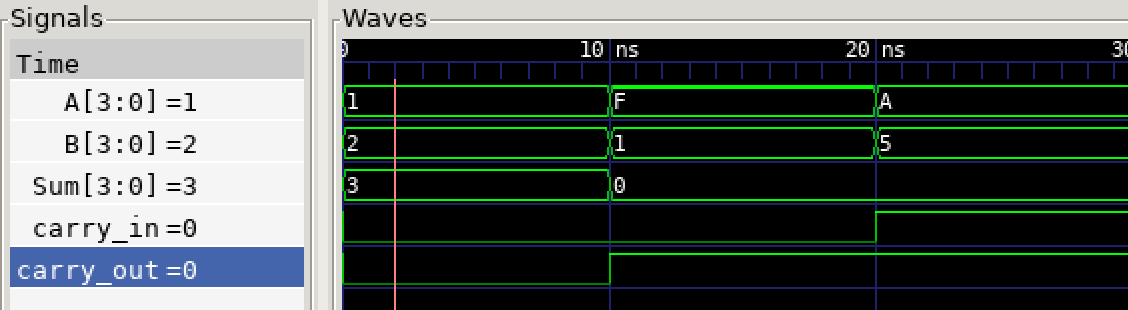
\includegraphics[width = 1.0\textwidth]{/Step2/Addition/addition_wave.png}
 \caption{Addition Circuit with marker at 2ns}
 \label{fig:enter-label} 
\end{figure} 

At 20ns, A=A(1010) and B=5(0101), so Sum=F(1111) with carry in & carry out at 0.
 \begin{figure}[h]
 \centering 
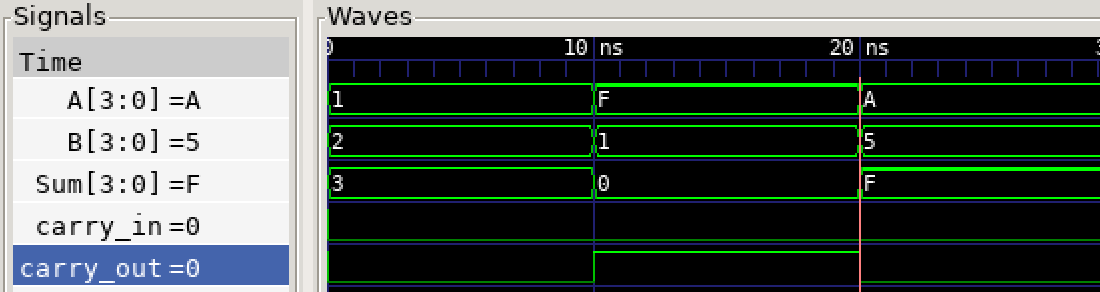
\includegraphics[width = 1.0\textwidth]{/Step2/Addition/addition_wave1.png}
 \caption{Addition Circuit with marker at 20ns}
 \label{fig:enter-label}
 \end{figure}

At 30ns, A & B are both 8(1000), so Sum=1 with carry in & carry out at 1, resulting in a decimal value of 17.
 \begin{figure}[h]
 \centering 
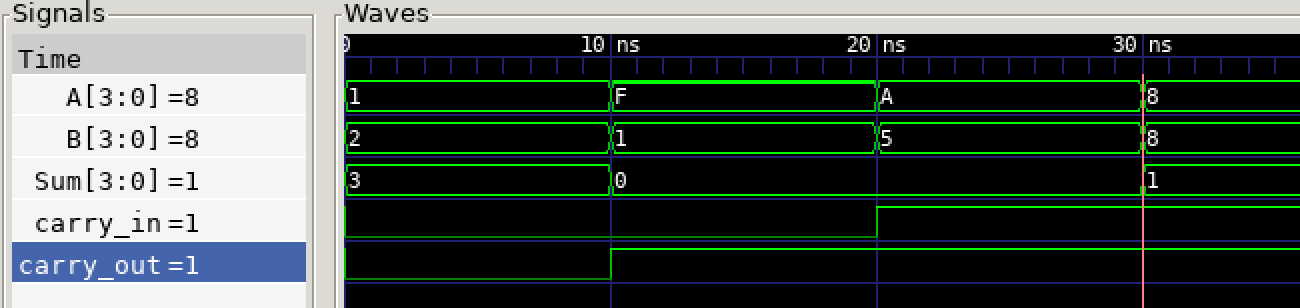
\includegraphics[width = 1.0\textwidth]{/Step2/Addition/addition_wave2.png}
 \caption{Addition Circuit with marker at 30ns}
 \label{fig:enter-label}
 \end{figure}

\subsection{Multiplication Circuit}
The Multiplication circuit takes two 4-bit inputs A & B, and produces two 4-bit outputs, product_low and product_high, representing the high and low 4 bits of A * B. The circuit has an intermediary 8-bit variable, full_product, which is used to extract the low and high 4 bits of the product. First, full_product is assigned A * B. Then, product_low is assigned the first 4 bits of full_product. Then, product_high is assigned the last 4 bits of full_product. 
\lstinputlisting[language=Verilog]{Multiplication/multiplication.v} 

To test the Multiplication circuit, we have created two registers A & B,and two wires product_low & product_high. We then perform 5 tests with A & B at various values. We will know that the Multiplication circuit is working as expected if <product_low>,<product_high> produces correct results for every combination of A * B that we have tested. For example, if A = 1111 and B = 1111, then the expected result is product_high = 1110, product_low = 0001 for a decimal value of 225.
\lstinputlisting[language=Verilog]{Multiplication/multiplication_tb.v}

\subsection{Multiplication Circuit Waveform} 

At 2ns, A=2 and B=3, so product_higher=0 and product_lower=6. 
\begin{figure}[h]
 \centering
 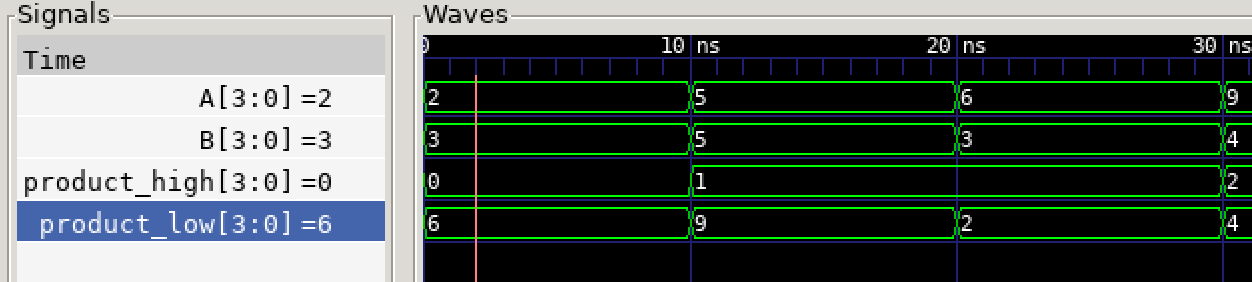
\includegraphics[width = 1.0\textwidth]{/Step2/Multiplication/multiplication_wave.png}
 \caption{Multiplication Circuit with marker at 2ns}
 \label{fig:enter-label} 
\end{figure} 

At 20ns, A=6 and B=3, so product_upper=0001 and product_lower=0010 for a decimal value of 18. 
 \begin{figure}[h]
 \centering 
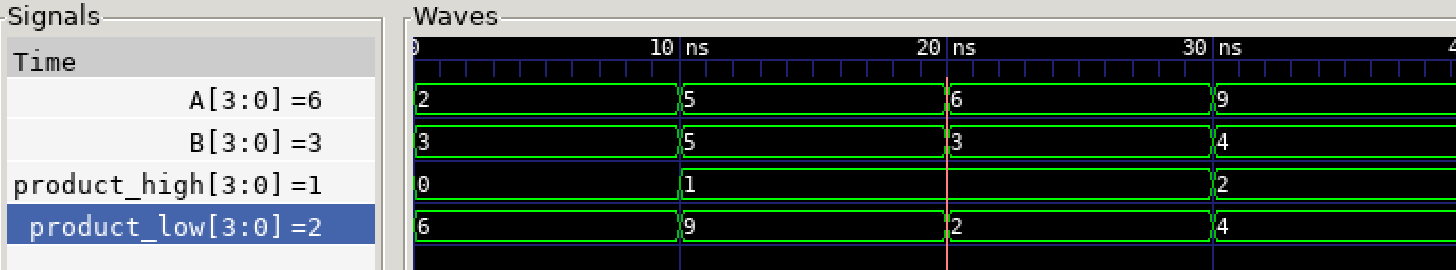
\includegraphics[width = 1.0\textwidth]{/Step2/Multiplication/multiplication_wave1.png}
 \caption{Multiplication Circuit with marker at 20ns}
 \label{fig:enter-label}
 \end{figure}

At 40ns, A & B are both F, so product_upper=E and product_lower=0001 for a decimal value of 256.
 \begin{figure}[h]
 \centering 
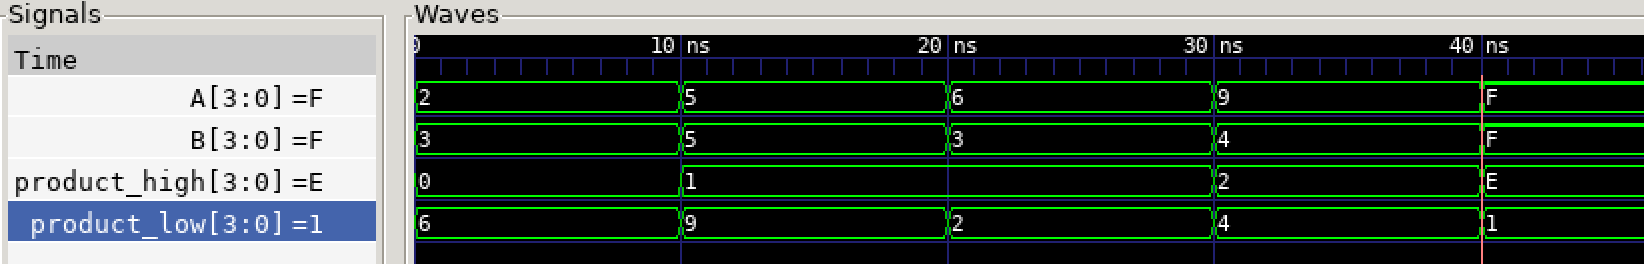
\includegraphics[width = 1.0\textwidth]{/Step2/Multiplication/multiplication_wave2.png}
 \caption{Multiplication Circuit with marker at 40ns}
 \label{fig:enter-label}
 \end{figure}


\section{Conclusion}

In Conclusion, we created 4 different circuits in Verilog and simulated them in GTKWave. The logic was quite trivial but the biggest trouble we ran into was getting all of the software set up on our respective systems. We worked well together as a group and learned quite a bit about the basics of verilog and GTKWave.
\end{document}



